\documentclass[11pt]{article}
\usepackage[a4paper,margin=2.25cm]{geometry}
\usepackage{fontspec}
\setmainfont{Times New Roman}
\setsansfont{Arial}
\usepackage{graphicx,booktabs,array,longtable,float,caption,cite,url,xurl,amsmath,amssymb}
\usepackage[hidelinks]{hyperref}
\captionsetup{font=small,labelfont=bf}
\setlength{\parskip}{0.35em}
\setlength{\parindent}{0pt}
\setlength{\emergencystretch}{3em}
\linespread{1.08}

\title{Recording-Grouped Bearing Fault Diagnosis under Directional Operating-Condition Shifts on the MCC5 Electric-Drive Benchmark}
\author{Yu Li\\Shanxi Engineering Vocational College, China}
\date{}
\begin{document}
\maketitle
\begin{abstract}
Windowed machinery benchmarks can overstate diagnostic transfer when correlated windows from one acquisition recording cross data partitions. We establish a recording-grouped benchmark on the MCC5-THU Motor bearing subset and examine transfer direction, partition sensitivity, feature membership, and acquisition-date structure. The study includes 84 recordings, 15,036 overlapping windows, and 254 numeric features; neural protocols use frozen recording roles and training-only z-score statistics. Across ten parallel split seeds, random assignment of overlapping windows yields 0.9976 $\pm$ 0.0009 macro-F1 while sharing all 84 source recordings between training and test, whereas recording-grouped assignment yields 0.9777 $\pm$ 0.0356 with zero source overlap. Leave-one-speed-out performance is directional: random-forest macro-F1 remains near 0.99 when 1000 or 2000 rpm is withheld but falls to 0.6921 for upward extrapolation from 1000/2000 to the nominal 3000-rpm domain. Recording-level aggregation preserves this boundary at 0.7020 macro-F1 over 28 test recordings. Same-date controls, including two severity-matched binary tasks, remain separable across ten recording-grouped splits, but training-only date metadata alone yields 0.7028--0.7723 macro-F1 across the four protocols. Because date is strongly associated with class and severity and physical specimen identifiers are unavailable, these controls support within-date fault-class separability but not session-independent diagnosis. The contribution is a direction-aware MCC5 benchmark, not evidence of specimen-, session-, or machine-independent generalization.
\end{abstract}
\noindent\textbf{Keywords:} bearing fault diagnosis; electric-drive monitoring; recording-grouped evaluation; directional transfer; speed extrapolation; multisource signals; MCC5-THU Motor

\section{Introduction}
Electric drives are central to manufacturing, transportation, and energy conversion, while bearing defects remain an important source of vibration, reliability loss, and unplanned downtime \cite{Lei2020Roadmap,Zio2021PHM,Fernandes2022IndustrialReview,Zonta2024AIPdM}. Data-driven bearing diagnosis now spans engineered vibration descriptors, motor-current analysis, convolutional and attention models, transfer learning, and domain generalization \cite{Zhang2020DLBearingReview,Neupane2020CWRUReview,Tama2022DLVibrationReview,Chen2023DeepTransferReview,Xiao2024DGSurvey}. The central deployment difficulty is not classification under randomly mixed laboratory windows, but diagnosis when speed, load, operating mode, acquisition session, or machine changes.

Localized bearing defects influence mechanical and electrical measurements differently. Vibration contains impacts, resonances, sidebands, and envelope modulation, whereas motor current reflects electromechanical coupling and torque-related modulation \cite{Gundewar2020InductionMotorReview,Toma2020MotorCurrentGA,Hoang2019MotorCurrentFusion,Guan2023MotorCurrentCausalConv}. Order-domain processing can align selected rotational components when speed varies, but its validity depends on pulse quality, angle resampling, amplitude normalization, and construction of a common order grid \cite{Lu2019TacholessReview,Jiang2023TacholessOrder,Duan2021AdaptiveTacholess,Ji2021OrderTracking1DCNN}. More recent domain-generalization studies learn invariant representations across machines and operating conditions, often with considerably broader validation than a single laboratory split \cite{Zhu2024DIRNet,Huang2025DPJDG}.

Evaluation provenance is equally consequential. Overlapping windows from one recording share sensor placement, background noise, control trajectory, and acquisition artifacts. Allowing those windows to cross data roles can inflate performance and underestimate uncertainty \cite{Kapoor2023Leakage,Hendriks2021CWRUBenchmark,Ragab2023AdaTime,Vieira2024ConnectomeLeakage,Wen2021MRILLeakage}. The MCC5 source article recommends recording-level separation before segmentation and training-side validation for unknown-condition evaluation \cite{Chen2026MCC5DataBrief,Chen2025MCC5Mendeley}. This study does not present recording grouping as a new algorithm. Instead, it operationalizes that principle as an auditable benchmark and asks four questions: (i) how sensitive are results to grouped partition choice; (ii) are operating-condition shifts symmetric in direction; (iii) what remains after exact feature membership replaces ambiguous substring groups; and (iv) which measured inputs are associated with apparent fusion gains under matched train-only standardization?

The contributions are threefold. First, a frozen recording-grouped MCC5 benchmark is reported with explicit transfer directions and a comparative analysis against random overlapping-window assignment. Second, repeated grouped partitions, a complete classical-model recording-level matrix, and class-stratified recording bootstrap distinguish partition, optimization, and finite-test-recording variability. Third, exact feature and input-schema audits are combined with raw-file identity, same-date, severity-matched, metadata-only, and date--severity composite controls. The resulting paper is a benchmark and sensitivity study, not a claim of universal model superiority.

\section{Related Work}
\subsection{Vibration, current, and order-aware diagnosis}
Traditional bearing diagnosis combines time statistics, spectral energy, envelope analysis, and characteristic-frequency reasoning. Traditional descriptors remain widely used alongside compact and physics-informed learning models, particularly when recording-level sample sizes are limited \cite{Hoang2018DLSurvey,Zhang2017CNNBearing,Ni2023PIResNet,Ruan2023CNNParameter}. Current-based diagnosis offers non-invasive electrical evidence but is sensitive to controller, supply, and loading conditions \cite{Gundewar2020InductionMotorReview,Toma2020MotorCurrentGA,Hoang2019MotorCurrentFusion,Guan2023MotorCurrentCausalConv}. Multisensor methods can exploit complementary signals, although benefit depends on branch definitions, scaling, and availability rather than the mere presence of more inputs \cite{Chen2017MultisensorSAE,Che2020HybridMultimodal,Wang2021ThreeStageFusion,Meng2023GraphAttentionFusion,You2024SoundVibrationPhysics,Xu2024HybridMultimodalFusion}.

Order tracking expresses spectral content relative to shaft rotation and is attractive for variable-speed diagnosis. Nevertheless, nominal frequency division, tachometer-assisted angular resampling, and truly normalized common-order grids are not equivalent. This distinction matters here because the existing engineered order fields include raw band sums and key-phase diagnostics; they are evaluated as explicit feature blocks and are not assumed to be speed invariant.

\subsection{Cross-mode learning and benchmark design}
Domain adaptation uses information from a target domain, while domain generalization learns from source domains without target access. Existing bearing methods include adversarial alignment, meta-learning, causal factorization, boundary-aware objectives, and physically informed representations \cite{Wan2022MultiAdversarialDA,Zhao2021JDAN,Li2021MetaLearningFewShot,Jia2023CausalFactorization,Li2022BoundaryDG,Pang2024FaultVibrationDG,Kim2023SingleDomainPI,Xie2024DualInvariantDG,Cheng2024CausalDG}. Their scientific claims depend strongly on split unit, direction, machine identity, and whether target data inform selection. The present work evaluates supervised baselines under fixed grouped protocols; it does not claim unsupervised adaptation or state-of-the-art DG performance.

\section{Materials and Methods}
\subsection{Dataset and diagnostic task}
MCC5-THU Motor was acquired on a 2.2 kW three-phase asynchronous motor connected to a torque sensor, gearbox, magnetic-powder brake, and synchronous acquisition system \cite{Chen2026MCC5DataBrief}. Eight channels contain key phase, torque, triaxial drive-end vibration, and three-phase current at 12.8 kHz for 90 s per recording. The bearing-only task pools light and high severities into healthy, inner-race, outer-race, and rolling-element labels. Pooling severity makes this a fault-location task and introduces within-class severity heterogeneity.

Raw-file provenance was audited against the official dataset copy without redistributing signal samples. For every catalogued recording, SHA-256, byte size, data shape, relative dataset path, and the acquisition timestamp encoded in the public filename were recorded. Repeated timestamps were examined by streaming value-level comparison. Acquisition dates were cross-tabulated with class and protocol role; Cramer's V, normalized mutual information, and an in-sample date-majority agreement were computed only as descriptive indicators of possible session confounding, not as diagnostic test performance.


\begin{table}[H]
\centering
\caption{MCC5 bearing-only data composition.}
\label{tab:dataset}
\small
\resizebox{\textwidth}{!}{%
\begin{tabular}{lcc}
\toprule
Item & Value & Interpretation \\
\midrule
Source recordings & 84 & 24 rolling-element; 23 inner-race; 25 outer-race; 12 healthy \\
Overlapping windows & 15,036 & 1.0 s window; 0.5 s stride; 179 windows per recording \\
Engineered feature table & 260 columns & 254 audited numeric candidates plus identifiers/labels \\
Signal channels & 8 & Key phase, torque, triaxial vibration, three-phase current \\
Sampling & 12.8 kHz, 90 s & Synchronous acquisition for each source recording \\
Physical bearing-instance identity & Not available in public metadata & Recording separation does not establish specimen independence \\
Raw-file identity audit & 84 distinct SHA-256 values & Excludes byte-identical files, not shared specimens or sessions \\
Acquisition dates & 5 & Date/class association is treated as descriptive confounding evidence \\
\bottomrule
\end{tabular}}

\end{table}


\begin{figure}[H]
\centering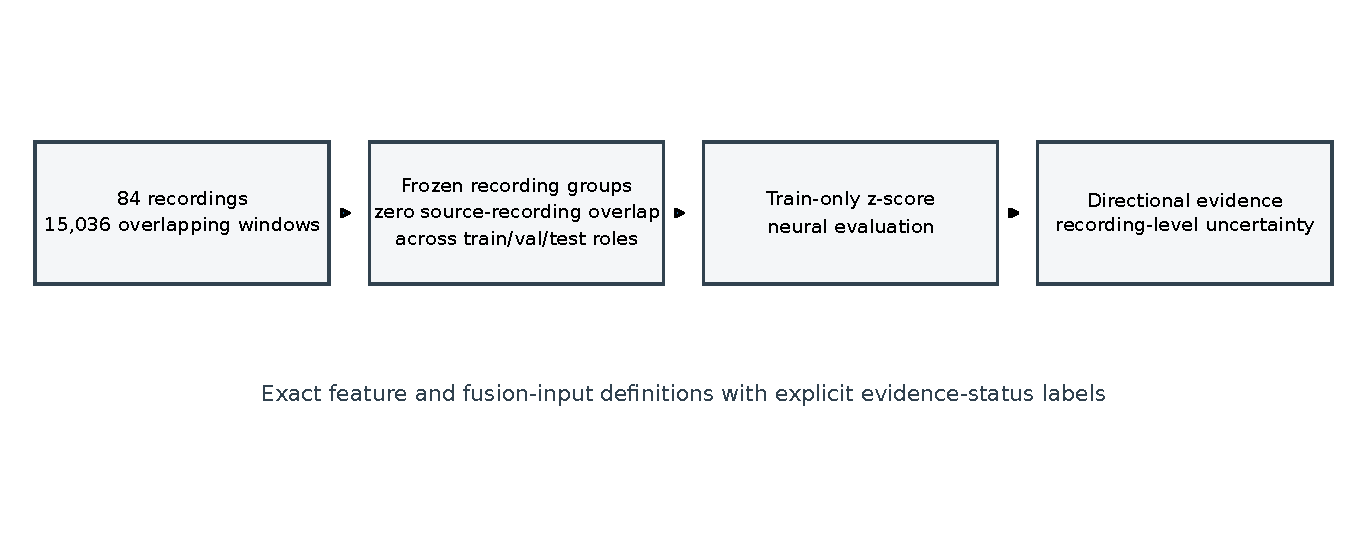
\includegraphics[width=0.96\textwidth]{figures/figure_1_workflow.pdf}
\caption{Overview of the recording-grouped MCC5 benchmark, from provenance-preserving segmentation and frozen recording roles to train-only preprocessing, directional evaluation, and recording-level uncertainty analysis.}
\label{fig:workflow}
\end{figure}

\subsection{Segmentation, feature schema, and raw inputs}
Each 90 s recording produces 179 one-second windows with a 0.5 s stride. Adjacent windows overlap by 50\%, so 15,036 windows are not treated as 15,036 independent experimental units. Engineered descriptors use all 12,800 samples. The audited feature table contains 254 numeric candidates: vibration time (36), vibration frequency (24), vibration envelope (15), vibration nominal order (27), vibration key-phase order/diagnostics (39), current time (36), current frequency (24), current nominal order (27), torque time (12), key-phase time (12), and RPM/load context (2).

The predefined raw-sequence protocol retains the first 8,192 samples (0.64 s); no resampling is performed. This input length was frozen before the standardized rerun to preserve architectural and computational comparability with the predefined neural benchmark. A matched sensitivity retains all 12,800 samples and is reported as a duration analysis rather than a post-hoc replacement of the primary protocol. Sequence statistics are fitted per channel on training windows only. Scalar missing values are imputed by training medians and standardized per feature with training means and standard deviations. Validation and test sets use the stored training statistics unchanged. Near-constant scales are replaced by one. Automated audits require transformed nonconstant training means within $10^{-3}$ of zero and standard deviations within $10^{-2}$ of one.

\subsection{Recording-grouped protocols}
All neural roles are frozen at source-recording level. The existing source-recording validation set is preserved; the other training sides allocate approximately 20\% of recordings per class to validation with seed 42. Windows from one source cannot cross roles, and no window-level fallback is permitted. The 3000-rpm test contains 28 recordings: 8 rolling-element, 7 inner-race, 9 outer-race, and 4 healthy.


\begin{table}[H]
\centering
\caption{Frozen recording-grouped neural evaluation roles.}
\label{tab:splits}
\small
\resizebox{\textwidth}{!}{%
\begin{tabular}{lccccc}
\toprule
Protocol & Train & Validation & Test & Train/val/test overlap & Window fallback \\
\midrule
Predefined grouped source-recording & 59 & 13 & 12 & 0 / 0 / 0 & No \\
Speed-circulation → torque-circulation & 34 & 8 & 42 & 0 / 0 / 0 & No \\
20 → 40 Nm & 34 & 8 & 42 & 0 / 0 / 0 & No \\
1000/2000 → 3000 rpm & 45 & 11 & 28 & 0 / 0 / 0 & No \\
\bottomrule
\end{tabular}}
\vspace{0.3em}\parbox{\textwidth}{\footnotesize Overlap entries are counts of shared source recordings across train/validation, train/test, and validation/test roles.}
\end{table}


The predefined directions are speed-circulation to torque-circulation (cross-mode), 20 to 40 Nm (cross-load), and 1000/2000 to 3000 rpm. Robustness checks reverse mode and load directions and evaluate each leave-one-RPM-out direction. Ten class-stratified recording-grouped partitions were generated with split seeds 42--51 while the classical-model seed was fixed at 42. Within each diagnostic class, approximately 70\%, 15\%, and 15\% of recordings were assigned to training, validation, and test roles; class-wise rounding yielded 59, 13, and 12 recordings, respectively, in every partition, with all four classes represented in each held-out test set. The fixed classical models used the training role and were evaluated once on the test role; the validation role was retained for protocol comparability.

\subsection{Models and fusion-input definitions}
Classical baselines include logistic regression, RBF-SVM, random forest, MLP, and XGBoost using training-side median imputation. Raw CNN, temporal convolutional network (TCN), and Transformer baselines use class-weighted cross-entropy, Adam with learning rate $10^{-3}$, batch size 64, at most 30 epochs, and patience 8. Each neural comparison uses the same frozen internal validation map. All preprocessing statistics and model-selection decisions were fitted exclusively on the training and internal-validation recordings. Classical and neural hyperparameters were fixed before final test evaluation; the held-out test recordings were not used for scaling, early stopping, or hyperparameter selection. Full settings are reported in the Supplementary Material and accompanying software supplement.

The branch network has vibration and current encoders, an optional scalar multilayer perceptron, sigmoid gating, and a classifier head. Six input definitions are distinguished: no scalar inputs; exactly RPM and load; a stored 26-field auxiliary bundle containing 24 waveform summaries (12 torque and 12 key-phase) plus two modality-presence indicators that are constant in this complete-modality subset; an auxiliary-context-28 bundle that adds RPM/load; a vibration-current network with a strict 254-feature engineered scalar branch (strict-254 scalar-branch fusion); and a legacy 262-field branch that additionally includes four window-position and four modality-availability fields. The 26/28-field settings were identified after inspecting the 3000-rpm holdout and are reported only as post-hoc exploratory evidence in the Supplementary Material.

\subsection{Metrics and uncertainty}
Macro-F1 is primary, worst-class recall identifies class collapse, and accuracy is supporting. Three optimization seeds are used generally and five for the focused 3000-rpm input audit. Seed standard deviation describes training variability only. For recording-level evaluation, window-level class probabilities are averaged within each test recording before assigning the recording label; majority vote is reported as a second aggregation rule. Class-stratified bootstrap resamples complete observed test recordings 2,000 times; overlapping windows are never sampled as independent units. The resulting empirical intervals are conditional on the fitted model and finite test-recording set and do not quantify performance on future specimens, sessions, or machines.

\subsection{Partition and session-proxy controls}
A direct partition control uses ten split seeds and a fixed XGBoost seed. Four protocols cross random versus recording-grouped assignment with overlapping 0.5-s-stride windows versus a nonoverlapping subset obtained by retaining every second window. The random protocols are intentionally invalid diagnostic estimates: they quantify the optimism that remains when windows from every source recording can occur on both sides of the split.

Four complementary controls use acquisition dates parsed from public recording identifiers. First, the 47 recordings acquired on 250707 provide a recording-grouped three-fault task; healthy recordings are unavailable on that date, and severity remains class-associated. Second, two severity-matched binary tasks on 250707 compare high-severity rolling-element versus outer-race faults and low-severity rolling-element versus inner-race faults. Random forest and XGBoost use all 254 descriptors over ten recording-grouped split seeds; each split contains only three and four test recordings, respectively. Third, date-only, operating-context-only, and combined metadata classifiers are fitted on the training recordings of each frozen protocol and evaluated on its test recordings. Fourth, acquisition date is predicted within the 25 outer-race recordings using ten repeated source-grouped folds and compared with a training-fold severity-majority rule. Because outer-race severity and date are strongly coupled, this is a date--severity composite control rather than an isolated test of session signatures. Its rarest date contains two recordings, so accuracy, macro-F1, and worst-class recall are reported together.

\section{Results}
\subsection{Raw-file identity and acquisition-date structure}
All 84 catalogue entries resolve to official raw files, and all 84 SHA-256 digests are distinct. One timestamp is shared by three filenames. Pairwise comparison across 1,152,000 rows and nine columns confirms a common time vector but different signal values for every pair; the anomaly therefore does not represent byte-identical or pointwise-identical signal files. This audit does not determine physical specimen identity or exclude transformed similarities.

The recordings span five acquisition dates, and class composition is uneven across them. An in-sample date-majority mapping agrees with 61 of 84 labels (0.7262), with Cramer's V of 0.7714 and normalized mutual information of 0.5989. The controls in Table~\ref{tab:session-controls} qualify this association. Both classical models separate the three same-date fault classes perfectly across ten grouped splits. The two severity-matched binary tasks are also perfectly separated by both models and both recording aggregations, although each split tests only three high-severity or four low-severity recordings. These results establish within-date fault-class separability for the observed binary contrasts, not specimen- or session-independent diagnosis. Training-only date metadata reaches 0.7028--0.7723 macro-F1 across the four frozen tests. Within outer-race recordings, the signal model reaches 0.5995 $\pm$ 0.0547 macro-F1 and zero worst-date recall, while a training-fold severity-majority rule reaches 0.6387 $\pm$ 0.0025 macro-F1 and likewise never recovers the rare date. The outer-race result therefore reflects date--severity composite predictability and does not independently establish session signatures.

\begin{table}[H]
\centering
\caption{Comparative partition and acquisition-date controls. Split variability uses ten split seeds with model seed 42. Same-date results use recording-level probability aggregation; the outer-race date task uses ten repeated source-grouped folds.}
\label{tab:session-controls}
\small
\resizebox{\textwidth}{!}{%
\begin{tabular}{lcccc}
\toprule
Control & Independent split unit & Source overlap & Reported metric & Result \\
\midrule
Random overlapping-window assignment & Window & 84 & Window macro-F1 & 0.9976 $\pm$ 0.0009 \\
Recording-grouped overlapping windows & Recording & 0 & Window macro-F1 & 0.9777 $\pm$ 0.0356 \\
Same-date 250707, three fault classes & Recording & 0 & Recording macro-F1 & 1.0000 $\pm$ 0.0000 \\
Same-date 250707, severity H, rolling-element vs. outer-race & Recording & 0 & Recording macro-F1 & 1.0000 (3 test records/split) \\
Same-date 250707, severity L, rolling-element vs. inner-race & Recording & 0 & Recording macro-F1 & 1.0000 (4 test records/split) \\
Date-only logistic baseline, four protocols & Recording & 0 & Recording macro-F1 range & 0.7028--0.7723 \\
Outer-race date--severity composite, signal model & Recording & 0 & Macro-F1 / worst recall & 0.5995 / 0.0000 \\
Outer-race date--severity composite, severity rule & Recording & 0 & Macro-F1 / worst recall & 0.6387 / 0.0000 \\
\bottomrule
\end{tabular}}
\end{table}

\subsection{Directional classical benchmark}
Classical feature models remain strong on source-recording, cross-mode, and cross-load protocols. Across ten grouped source-recording partitions, XGBoost reaches 0.9777 $\pm$ 0.0356 window-level macro-F1, with a range of 0.9092--0.9992; after probability aggregation within recording, it reaches 0.9829 $\pm$ 0.0361, with a range of 0.9143--1.0000. Direction changes the conclusion most strongly for speed. Holding out 1000 or 2000 rpm remains near 0.99, whereas holding out the nominal 3000-rpm domain reduces random-forest macro-F1 to 0.6921 and worst-class recall to 0.1099.


\begin{table}[H]
\centering
\caption{Directional robustness of the fixed 254-feature random-forest baseline.}
\label{tab:directional}
\small
\resizebox{\textwidth}{!}{%
\begin{tabular}{lcccc}
\toprule
Held-out direction & Model & Macro-F1 & Worst recall & Accuracy \\
\midrule
Speed-circulation → torque-circulation & Random forest & 0.9790 & 0.9167 & 0.9761 \\
Torque-circulation → speed-circulation & Random forest & 0.9379 & 0.8822 & 0.9307 \\
20 → 40 Nm & Random forest & 0.9891 & 0.9795 & 0.9891 \\
40 → 20 Nm & Random forest & 0.9564 & 0.8457 & 0.9507 \\
Hold out 1000 rpm & Random forest & 0.9908 & 0.9860 & 0.9906 \\
Hold out 2000 rpm & Random forest & 0.9973 & 0.9951 & 0.9974 \\
Hold out 3000 rpm & Random forest & 0.6921 & 0.1099 & 0.6983 \\
\bottomrule
\end{tabular}}

\end{table}


\begin{figure}[H]
\centering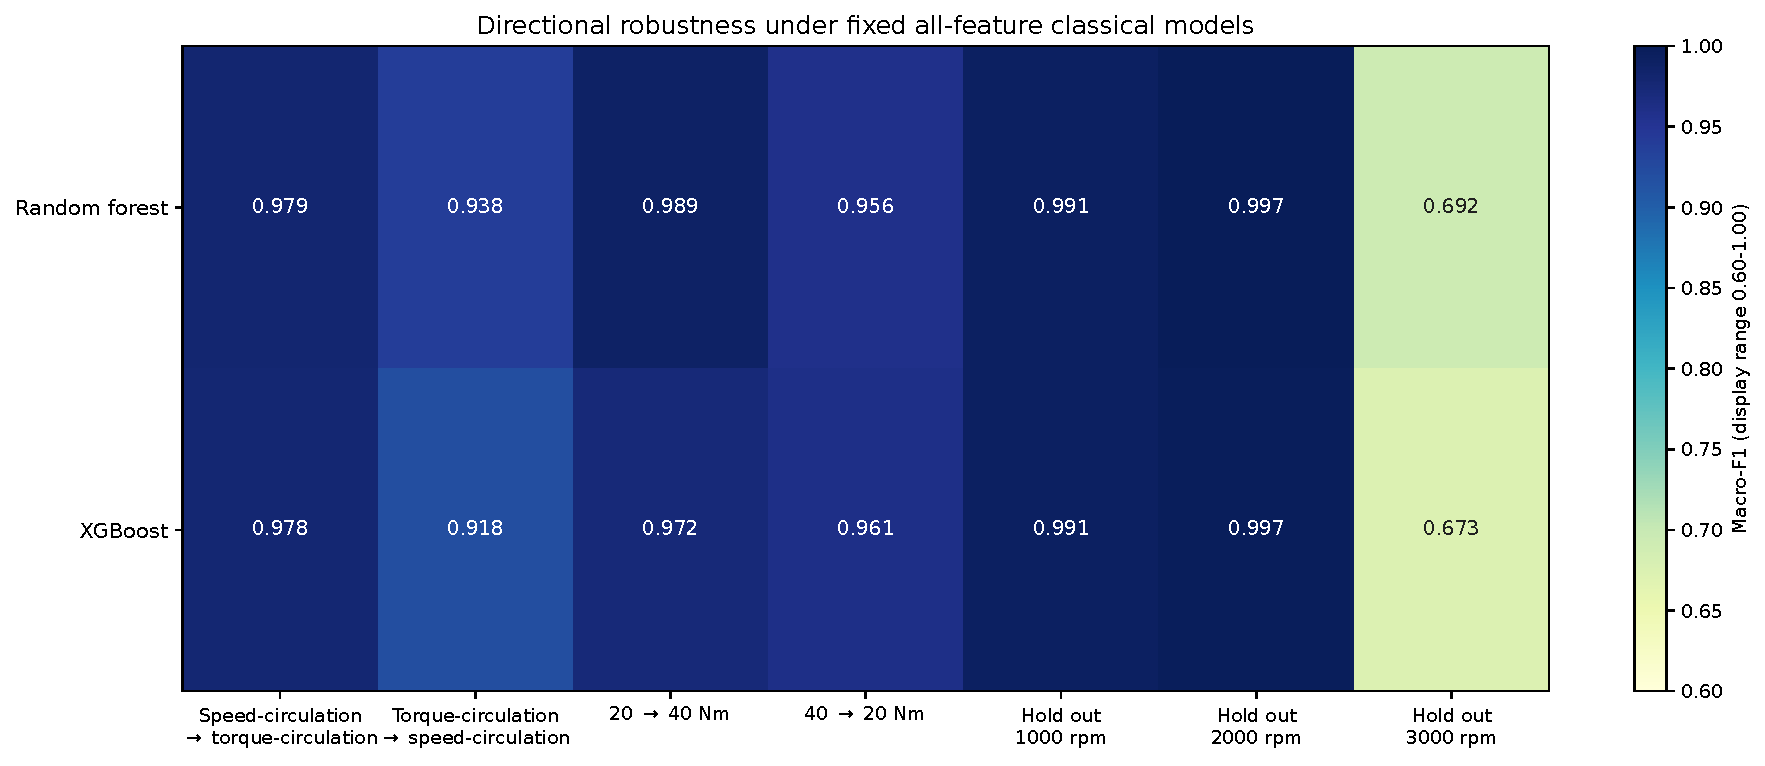
\includegraphics[width=0.98\textwidth]{figures/figure_2_directional_robustness.pdf}
\caption{Directional robustness under fixed all-feature classical models. The displayed color range is restricted to 0.60--1.00 to make differences among the seven directional protocols visible.}
\label{fig:directional}
\end{figure}

\begin{figure}[H]
\centering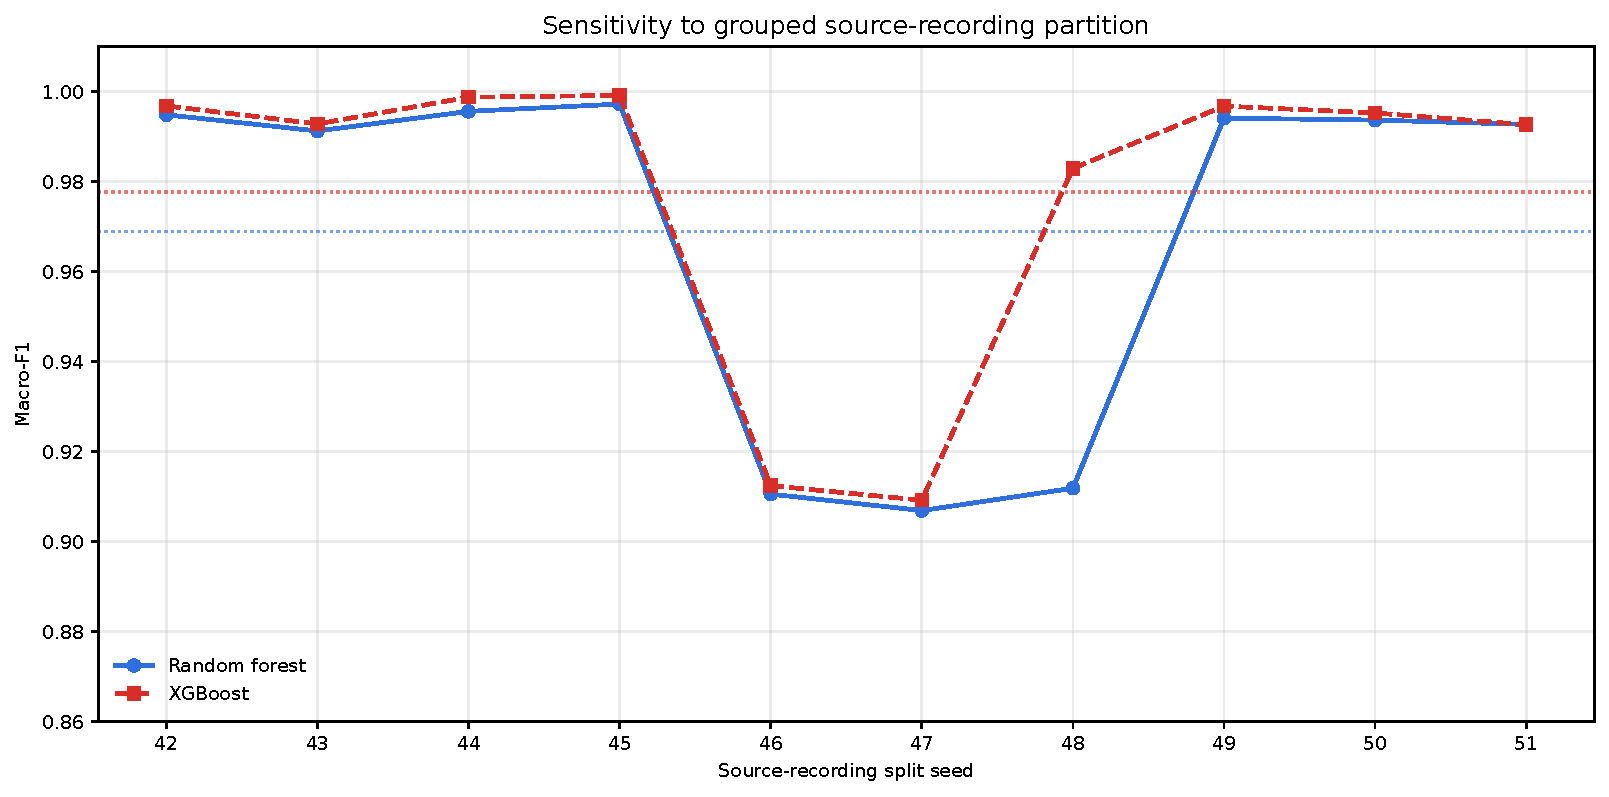
\includegraphics[width=0.98\textwidth]{figures/figure_3_partition_sensitivity.pdf}
\caption{Sensitivity to ten class-stratified grouped source-recording partitions generated with split seeds 42--51. The classical-model seed is fixed at 42; variation therefore reflects partition choice rather than optimization randomness. Random forest uses a solid line with circular markers, whereas XGBoost uses a dashed line with square markers. Dotted horizontal lines denote the model-specific means across the ten partitions, and the vertical axis is restricted to 0.86--1.01. Each partition contains 59 training, 13 validation, and 12 test recordings, with all four classes represented in the test role.}
\label{fig:partition}
\end{figure}

\subsection{Exact feature definitions}
An exact membership audit shows that the former substring-defined groups mixed time, frequency, envelope, and order fields. Those legacy rows are retained only as provenance. Under exact grouping on the 3000-rpm holdout, XGBoost reaches 0.7569 with all non-order signal descriptors, 0.7556 after RPM/load is added, and 0.7596 after nominal-order fields are added. Full key-phase/order inclusion reduces the all-feature XGBoost score to 0.6733. Thus, non-order multisignal descriptors carry most aggregate high-speed performance, while the current order implementation does not establish speed invariance.

\begin{figure}[H]
\centering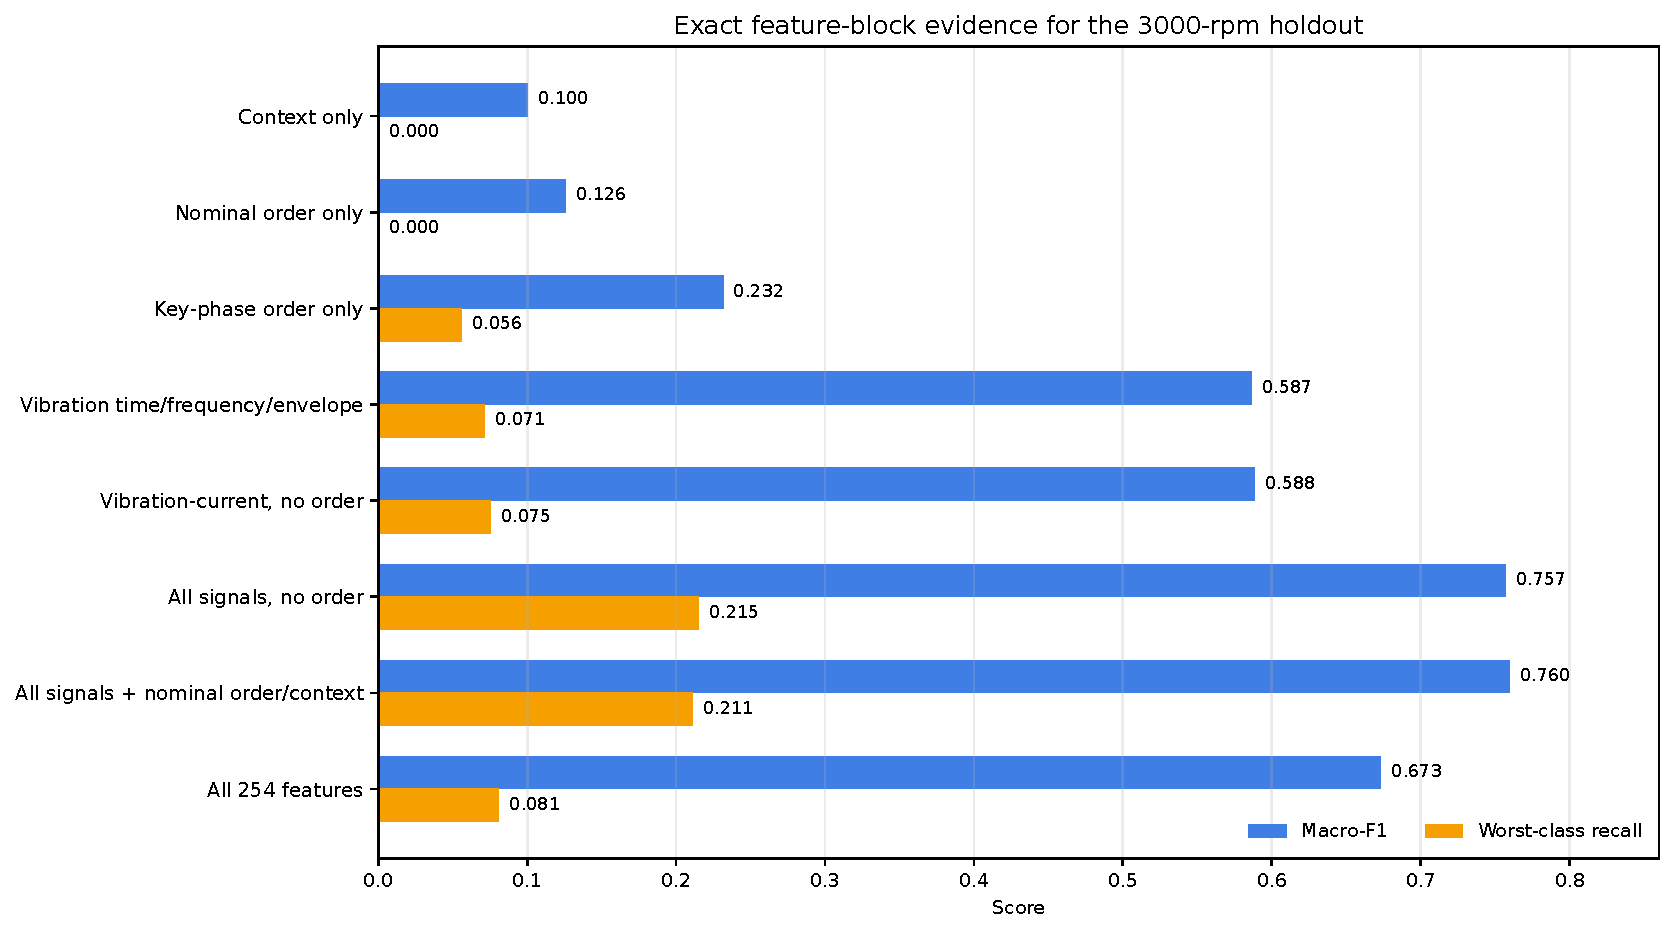
\includegraphics[width=0.98\textwidth]{figures/figure_4_exact_feature_blocks.pdf}
\caption{Exact feature-block evidence for the 3000-rpm holdout. Numeric labels report macro-F1 and worst-class recall for every feature definition, including zero-valued worst-class recall.}
\label{fig:features}
\end{figure}

\subsection{Raw neural baselines}
Under train-only per-channel standardization, the Transformer reaches 0.9531 $\pm$ 0.0289 macro-F1 on source-recording evaluation. Cross-mode CNN, TCN, and Transformer means are all between 0.9356 and 0.9501. At 3000 rpm, however, CNN falls to 0.6644 $\pm$ 0.1523; TCN and Transformer fall further. Validation macro-F1 remains close to one, highlighting the mismatch between known-condition validation and unseen high-speed test data.


\begin{table}[H]
\centering
\caption{Raw vibration-current models with train-only per-channel standardization.}
\label{tab:raw}
\small
\resizebox{\textwidth}{!}{%
\begin{tabular}{lcccc}
\toprule
Protocol & Model & Macro-F1 mean ± SD & Worst recall mean ± SD & Seeds \\
\midrule
Source-recording & CNN & 0.8535 ± 0.0286 & 0.5768 ± 0.0631 & 3 \\
Source-recording & TCN & 0.8759 ± 0.0263 & 0.5964 ± 0.0840 & 3 \\
Source-recording & Transformer & 0.9531 ± 0.0289 & 0.8762 ± 0.0804 & 3 \\
Cross-mode & CNN & 0.9501 ± 0.0076 & 0.8703 ± 0.0506 & 3 \\
Cross-mode & TCN & 0.9432 ± 0.0115 & 0.8749 ± 0.0367 & 3 \\
Cross-mode & Transformer & 0.9356 ± 0.0092 & 0.8915 ± 0.0320 & 3 \\
Cross-load & CNN & 0.8750 ± 0.0256 & 0.7337 ± 0.0839 & 3 \\
Cross-load & TCN & 0.7302 ± 0.0989 & 0.3726 ± 0.1638 & 3 \\
Cross-load & Transformer & 0.9076 ± 0.0602 & 0.7981 ± 0.1276 & 3 \\
1000/2000 → 3000 rpm & CNN & 0.6644 ± 0.1523 & 0.4270 ± 0.2296 & 3 \\
1000/2000 → 3000 rpm & TCN & 0.5011 ± 0.0465 & 0.2381 ± 0.1018 & 3 \\
1000/2000 → 3000 rpm & Transformer & 0.4703 ± 0.0810 & 0.1932 ± 0.0463 & 3 \\
\bottomrule
\end{tabular}}

\end{table}


\begin{figure}[H]
\centering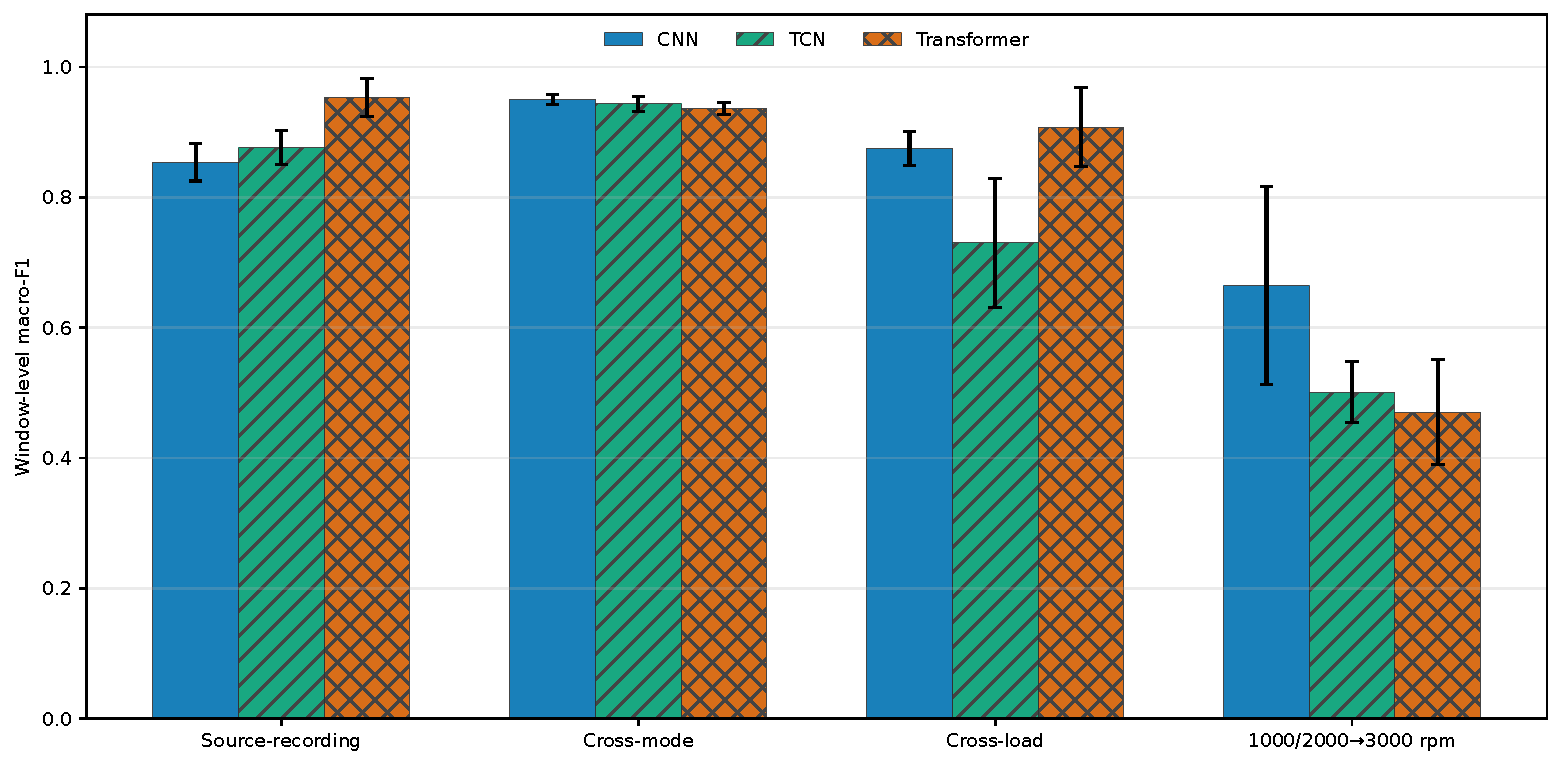
\includegraphics[width=0.92\textwidth]{figures/figure_5_corrected_raw_models.pdf}
\caption{Raw-model macro-F1 with train-only standardization. Error bars are optimization-seed standard deviations ($n=3$); bar hatching distinguishes model families in grayscale.}
\label{fig:raw}
\end{figure}

\subsection{Fusion-input audit}
With train-only standardization, strict-254 scalar-branch fusion reaches 0.9939, 0.9723, and 0.9299 mean macro-F1 on source-recording, cross-mode, and cross-load protocols, respectively. It falls to 0.4001 $\pm$ 0.0813 on the 3000-rpm holdout, where its worst-class recall is near zero.

The predefined focused input audit separates signal roles. No-scalar and RPM/load-only branches reach 0.7081 and 0.7124 mean macro-F1, respectively, so nominal RPM/load alone does not materially change the high-speed result under this matched protocol. The 26/28-field bundles were selected after viewing the same holdout; all of their numerical evidence is therefore confined to the Supplementary Material as hypothesis-generating disclosure.


\begin{table}[H]
\centering
\caption{Predefined input-definition audit for the 1000/2000-to-3000-rpm holdout. Values are means and standard deviations across five optimization seeds. Post-hoc 26/28-field configurations are excluded and reported only in the Supplementary Material.}
\label{tab:fusion}
\small
\resizebox{\textwidth}{!}{%
\begin{tabular}{lcccc}
\toprule
Configuration & Scalar inputs & Macro-F1 mean ± SD & Worst recall mean ± SD & Evidence status \\
\midrule
Vibration-current; no scalars & 0 & 0.7081 ± 0.0986 & 0.4324 ± 0.1507 & Matched protocol \\
Vibration-current + RPM/load & 2 & 0.7124 ± 0.0529 & 0.4272 ± 0.0964 & Matched protocol \\
Strict-254 scalar-branch fusion & 254 & 0.4001 ± 0.0813 & 0.0257 ± 0.0045 & Matched protocol \\
\bottomrule
\end{tabular}}
\end{table}


\subsection{Recording-level evidence and input duration}
Recording aggregation exposes class-level fragility that window counts can obscure. Table~\ref{tab:classical-source} reports the predefined primary classical model for every protocol; the complete five-model by four-protocol matrix is provided in the Supplementary Material. Mean-probability aggregation remains perfect on the predefined source-recording and cross-load tests and reaches 0.9791 macro-F1 for cross-mode transfer. On the nominal 3000-rpm domain, however, it falls to 0.7020 macro-F1 with a worst-class recall of 0.1111; majority voting falls to 0.6444 macro-F1 and zero worst-class recall. The full matrix confirms model dependence: recording-level macro-F1 ranges from 0.1585 to 0.7020 on this protocol.

\begin{table}[H]
\centering
\caption{Classical source-recording evaluation. Intervals are class-stratified 95\% empirical recording-resampling intervals over 2,000 replicates, conditional on the fitted model and observed test recordings. Majority vote is reported as a sensitivity aggregation.}
\label{tab:classical-source}
\small
\resizebox{\textwidth}{!}{%
\begin{tabular}{llccccc}
\toprule
Protocol & Model & Test recordings & Mean-probability macro-F1 & 95\% interval & Majority-vote macro-F1 & Mean-probability worst recall \\
\midrule
Predefined source-recording & XGBoost & 12 & 1.0000 & [1.0000, 1.0000] & 1.0000 & 1.0000 \\
Cross-mode & Random forest & 42 & 0.9791 & [0.9365, 1.0000] & 0.9791 & 0.9167 \\
Cross-load & Random forest & 42 & 1.0000 & [1.0000, 1.0000] & 1.0000 & 1.0000 \\
1000/2000 to 3000 rpm & Random forest & 28 & 0.7020 & [0.6355, 0.8000] & 0.6444 & 0.1111 \\
\bottomrule
\end{tabular}}
\end{table}

Degenerate intervals such as [1.0000, 1.0000] mean that resampling the observed finite test recordings did not change the empirical score. They do not imply zero uncertainty for future bearings, acquisition sessions, or machines.

For the corrected neural and fusion models, strict-254 scalar-branch fusion has zero recording-level worst-class recall on every seed at 3000 rpm. All values in Table~\ref{tab:source} are based on 28 test recordings rather than thousands of correlated windows; post-hoc auxiliary-bundle results remain in the Supplementary Material.


\begin{table}[H]
\centering
\caption{Recording-level mean-probability aggregation on the 3000-rpm holdout. Raw-CNN values use three optimization seeds; focused fusion-branch values use five. Means and standard deviations are calculated after aggregation within each recording; recording-cluster bootstrap intervals are reported separately in the Supplementary Material.}
\label{tab:source}
\small
\resizebox{\textwidth}{!}{%
\begin{tabular}{lcccc}
\toprule
Model/configuration & Test recordings & Seeds & Recording macro-F1 mean ± SD & Recording worst recall mean ± SD \\
\midrule
Raw CNN & 28 & 3 & 0.7233 ± 0.2492 & 0.4722 ± 0.4111 \\
No-scalar branch & 28 & 5 & 0.7122 ± 0.1238 & 0.4000 ± 0.2054 \\
RPM/load branch & 28 & 5 & 0.7306 ± 0.0917 & 0.4000 ± 0.1369 \\
Strict-254 scalar-branch fusion & 28 & 5 & 0.3660 ± 0.1254 & 0.0000 ± 0.0000 \\
\bottomrule
\end{tabular}}

\end{table}


Retaining the complete one-second raw sequence raises CNN window-level macro-F1 from 0.6644 to 0.7187 and reduces seed variability, but the high-speed boundary remains. This matched sensitivity isolates retained duration without changing architecture or split; it does not replace the frozen 8,192-sample primary protocol after observing the test result.


\begin{table}[H]
\centering
\caption{Matched raw-CNN input-length sensitivity on the 3000-rpm holdout.}
\label{tab:length}
\small
\resizebox{\textwidth}{!}{%
\begin{tabular}{lccc}
\toprule
Retained samples & Macro-F1 mean ± SD & Worst recall mean ± SD & Batched inference time (ms/window) \\
\midrule
8192 & 0.6644 ± 0.1523 & 0.4270 ± 0.2296 & 0.0432 \\
12800 & 0.7187 ± 0.0578 & 0.4986 ± 0.1657 & 0.0661 \\
\bottomrule
\end{tabular}}
\vspace{0.3em}\parbox{\textwidth}{\footnotesize Inference time was measured on an NVIDIA GeForce RTX 5080 over one complete test-set pass per optimization seed, using batch size 64 and no dedicated warm-up. The timer includes batched DataLoader iteration, host-to-device transfer, softmax, and output transfer to the host, but excludes disk I/O and preprocessing. Values are means across three seeded passes.}
\end{table}


\section{Discussion}
\subsection{What recording grouping establishes}
Recording grouping removes direct sharing of overlapping windows across data roles. It does not establish independent physical bearing specimens because the public metadata do not provide a verifiable bearing-instance identifier. The protocol is therefore described specifically as recording-grouped, without making a broader leakage-safety claim. Results are limited to the MCC5 bearing-only subset and should not be interpreted as cross-machine validation.

Raw-file hashing excludes byte-identical recordings, including within the repeated-timestamp group, but it does not resolve shared specimen or session identity. The same-date three-class and severity-matched binary controls show that the observed fault locations remain separable when date, and in the binary tasks severity, are fixed. Their test sets are small and repeatedly resample the same finite recordings. Conversely, date-only metadata retains label information. Outer-race date prediction does not isolate session structure because severity alone predicts date more accurately than the signal model. Recording grouping therefore removes direct window sharing, but the available controls cannot establish independence from specimen, severity, or session structure.

\subsection{Why upward high-speed extrapolation is different}
The asymmetry among the leave-one-speed-out tests is the central engineering result. Interpolation to 2000 rpm and downward extrapolation to 1000 rpm remain easy for the engineered classical models, but upward extrapolation to 3000 rpm produces class collapse for several otherwise strong models. This is consistent with a support-boundary problem: the test speed lies beyond the training range, and spectral distributions, amplitudes, controller behavior, and signal-to-noise relationships can all change together.

\subsection{Order-aware is not automatically speed invariant}
Frequency-to-order mapping is physically meaningful, yet raw order-band sums and imperfect key-phase estimates do not guarantee a common invariant representation. The exact block results support only a narrow conclusion: nominal-order features offer a small aggregate increment in one configuration, while order-only and full key-phase-order blocks are weak. A stronger order claim requires pulse-quality gating, robust interval filtering, fixed samples per revolution, common-grid interpolation, and density-normalized bands.

\subsection{What the fusion-input audit supports}
The predefined input audit supports two distinctions. First, strict-254 scalar-branch fusion performs strongly on three protocols with train-only z-score scaling but remains weak on the 3000-rpm holdout; this does not support a general claim that multisource fusion is defective. Second, adding RPM/load to the vibration-current branch produces little change under the high-speed protocol. A separate post-hoc audit of stored 26/28-field bundles is disclosed only in the Supplementary Material. Two stored presence indicators are constant here, leaving 24 varying torque/key-phase summaries; same-holdout discovery precludes a confirmatory interpretation regardless of their observed performance.

\subsection{Implications for benchmark reporting}
MCC5 studies should report the source recording as the split unit, provide transfer direction, distinguish train-seed variability from partition variability and conditional recording-resampling intervals, list exact input columns, and disclose whether candidate selection touched the test condition. The random-versus-grouped control demonstrates that merely discarding overlapping windows does not prevent source leakage: every recording still crosses roles under random nonoverlapping-window assignment. Window-level metrics remain useful for local diagnostic behavior, but they should be accompanied by recording-level results and a complete model matrix whenever windows overlap.

\section{Limitations}
The study uses one controlled rig and one bearing subset. Physical specimen identity is not available, severity levels are pooled, and no external machine or independent bearing set is harmonized sufficiently for confirmatory validation. Five acquisition dates are unevenly associated with class (Cramer's V 0.7714). The same-date controls omit healthy recordings, cover one date, and test only three or four recordings per severity-matched split. Outer-race date prediction is confounded by severity and has only two recordings on its rarest date. These controls characterize, but cannot remove, the remaining specimen/session ambiguity. The 26/28-field auxiliary configurations are post-hoc. Neural seed counts are modest, and classical directional experiments use fixed hyperparameters rather than nested optimization. The strict full branch still uses a compact architecture; its 3000-rpm failure does not imply that all fusion strategies will fail.

The engineered order features do not yet use a fully normalized common order grid, and key-phase quality requires stronger gating. Raw data remain in sensor-voltage units in the processed table. Future work should confirm auxiliary-signal findings on a locked dataset, add a protocol-matched modern domain-generalization baseline, and test independent devices or specimens.

\section{Conclusions}
This study provides a recording-grouped MCC5 bearing benchmark with explicit operating-shift direction and train-only standardization. Comparative partition controls show that random window assignment gives uniformly optimistic results while allowing every recording to cross roles; recording grouping lowers the mean modestly but exposes much larger variation among held-out recordings. Classical models remain strong on source-recording, cross-mode, and cross-load protocols, while upward extrapolation from 1000/2000 to the nominal 3000-rpm domain is the dominant boundary across classical and neural evidence.

The input audit also clarifies the fusion interpretation. Strict-254 scalar-branch fusion is strong on easier protocols but collapses at 3000 rpm, while RPM/load alone adds little to the vibration-current branch. Same-date and severity-matched controls retain fault-class separability, yet metadata-only and date--severity composite controls expose unresolved dataset structure. Post-hoc auxiliary-bundle results are retained only as transparent Supplementary evidence and do not support model superiority. The contribution is therefore a reproducible directional benchmark and sensitivity audit, not proof of specimen independence, universal order invariance, session-independent diagnosis, or confirmatory auxiliary-fusion superiority.

\section*{Data Availability Statement}
The MCC5-THU Motor data are publicly available through the original Mendeley Data record \cite{Chen2025MCC5Mendeley} and are not redistributed. Versioned code, frozen source-recording split maps, exact input schemas, result tables, reproduction scripts, and a compact raw-file audit containing relative paths, shapes, and SHA-256 digests for all 84 catalogued recordings are publicly available at \url{https://github.com/YOMMMO/mcc5-bearing-paper-review/releases/tag/review-v3.1.5}.

\section*{Author Contributions}
Yu Li: Conceptualization, methodology, software, validation, formal analysis, investigation, data curation, visualization, writing, and project administration.

\section*{Funding}
This research received no external funding.

\section*{Institutional Review Board Statement}
Not applicable. The study uses machinery signals and involves no human or animal participants.

\section*{Conflicts of Interest}
The author declares no conflict of interest.

\section*{Use of Generative AI}
During manuscript and software preparation from 9 July to 28 August 2026, the author used OpenAI ChatGPT Pro for reviewer-style critique and English-editing suggestions and OpenAI Codex for code review, implementation assistance, documentation, and local consistency checks. These tools did not generate or alter the raw measurements. All analyses were executed locally; the author inspected the code changes, selected the final analyses and interpretations, and verified the reported values, figures, and references against saved artifacts. The author takes full responsibility for the content of this publication.

\begin{thebibliography}{99}
\bibitem{Lei2020Roadmap} Lei, Yaguo; Yang, Bin; Jiang, Xinwei; Jia, Feng; Li, Naipeng; Nandi, Asoke K. Applications of machine learning to machine fault diagnosis: A review and roadmap. Mechanical Systems and Signal Processing. 2020; 138: 106587. doi:\url{10.1016/j.ymssp.2019.106587}.

\bibitem{Zio2021PHM} Zio, Enrico. Prognostics and Health Management (PHM): Where are we and where do we (need to) go in theory and practice. Reliability Engineering \& System Safety. 2022; 218: 108119. doi:\url{10.1016/j.ress.2021.108119}.

\bibitem{Fernandes2022IndustrialReview} Fernandes, Marta; Corchado, Juan Manuel; Marreiros, Goreti. Machine learning techniques applied to mechanical fault diagnosis and fault prognosis in the context of real industrial manufacturing use-cases: a systematic literature review. Applied Intelligence. 2022; 52(12): 14246-14280. doi:\url{10.1007/s10489-022-03344-3}.

\bibitem{Zonta2024AIPdM} Ucar, Aysegul; Karakose, Mehmet; Krmca, Necim. Artificial Intelligence for Predictive Maintenance Applications: Key Components, Trustworthiness, and Future Trends. Applied Sciences. 2024; 14(2): 898. doi:\url{10.3390/app14020898}.

\bibitem{Zhang2020DLBearingReview} Zhang, Shen; Zhang, Shibo; Wang, Bingnan; Habetler, Thomas G. Deep Learning Algorithms for Bearing Fault Diagnostics-A Comprehensive Review. IEEE Access. 2020; 8: 29857-29881. doi:\url{10.1109/access.2020.2972859}.

\bibitem{Neupane2020CWRUReview} Neupane, Dhiraj; Seok, Jongwon. Bearing Fault Detection and Diagnosis Using Case Western Reserve University Dataset With Deep Learning Approaches: A Review. IEEE Access. 2020; 8: 93155-93178. doi:\url{10.1109/access.2020.2990528}.

\bibitem{Tama2022DLVibrationReview} Tama, Bayu Adhi; Vania, Malinda; Lee, Seungchul; Lim, Sunghoon. Recent advances in the application of deep learning for fault diagnosis of rotating machinery using vibration signals. Artificial Intelligence Review. 2023; 56(5): 4667-4709. doi:\url{10.1007/s10462-022-10293-3}.

\bibitem{Chen2023DeepTransferReview} Chen, Xiaohan; Yang, Rui; Xue, Yihao; Huang, Mengjie; Ferrero, Roberto; Wang, Zidong. Deep Transfer Learning for Bearing Fault Diagnosis: A Systematic Review Since 2016. IEEE Transactions on Instrumentation and Measurement. 2023; 72: 1-21. doi:\url{10.1109/tim.2023.3244237}.

\bibitem{Xiao2024DGSurvey} Xiao, Yiming; Shao, Haidong; Yan, Shen; Wang, Jie; Peng, Ying; Liu, Bin. Domain generalization for rotating machinery fault diagnosis: A survey. Advanced Engineering Informatics. 2025; 64: 103063. doi:\url{10.1016/j.aei.2024.103063}.

\bibitem{Gundewar2020InductionMotorReview} Gundewar, Swapnil K.; Kane, Prasad V. Condition Monitoring and Fault Diagnosis of Induction Motor. Journal of Vibration Engineering \& Technologies. 2021; 9(4): 643-674. doi:\url{10.1007/s42417-020-00253-y}.

\bibitem{Toma2020MotorCurrentGA} Toma, Rafia Nishat; Prosvirin, Alexander E.; Kim, Jong-Myon. Bearing Fault Diagnosis of Induction Motors Using a Genetic Algorithm and Machine Learning Classifiers. Sensors. 2020; 20(7): 1884. doi:\url{10.3390/s20071884}.

\bibitem{Hoang2019MotorCurrentFusion} Hoang, Duy Tang; Kang, Hee Jun. A Motor Current Signal-Based Bearing Fault Diagnosis Using Deep Learning and Information Fusion. IEEE Transactions on Instrumentation and Measurement. 2020; 69(6): 3325-3333. doi:\url{10.1109/tim.2019.2933119}.

\bibitem{Guan2023MotorCurrentCausalConv} Guan, Bokai; Bao, Xiaohua; Qiu, Haotian; Yang, Dongliang. Enhancing bearing fault diagnosis using motor current signals: A novel approach combining time shifting and CausalConvNets. Measurement. 2024; 226: 114049. doi:\url{10.1016/j.measurement.2023.114049}.

\bibitem{Lu2019TacholessReview} Lu, Siliang; Yan, Ruqiang; Liu, Yongbin; Wang, Qunjing. Tacholess Speed Estimation in Order Tracking: A Review With Application to Rotating Machine Fault Diagnosis. IEEE Transactions on Instrumentation and Measurement. 2019; 68(7): 2315-2332. doi:\url{10.1109/tim.2019.2902806}.

\bibitem{Jiang2023TacholessOrder} Jiang, Zuhua; Zhang, Kun; Zhang, Xiangfeng; Xu, Yonggang. A Tacholess Order Tracking Method Based on Spectral Amplitude Modulation for Variable Speed Bearing Fault Diagnosis. IEEE Transactions on Instrumentation and Measurement. 2023; 72: 1-8. doi:\url{10.1109/tim.2023.3280512}.

\bibitem{Duan2021AdaptiveTacholess} Duan, Rongkai; Liao, Yuhe; Yang, Lei. Adaptive tacholess order tracking method based on generalized linear chirplet transform and its application for bearing fault diagnosis. ISA Transactions. 2022; 127: 324-341. doi:\url{10.1016/j.isatra.2021.08.039}.

\bibitem{Ji2021OrderTracking1DCNN} Ji, Mengyu; Peng, Gaoliang; He, Jun; Liu, Shaohui; Chen, Zhao; Li, Sijue. A Two-Stage, Intelligent Bearing-Fault-Diagnosis Method Using Order-Tracking and a One-Dimensional Convolutional Neural Network with Variable Speeds. Sensors. 2021; 21(3): 675. doi:\url{10.3390/s21030675}.

\bibitem{Zhu2024DIRNet} Zhu, Q.; Liu, H.; Bao, C.; Zhu, J.; Mao, X.; He, S.; Peng, F. Decoupled interpretable robust domain generalization networks: A fault diagnosis approach across bearings, working conditions, and artificial-to-real scenarios. \textit{Advanced Engineering Informatics} \textbf{2024}, \textit{61}, 102445. doi:\url{10.1016/j.aei.2024.102445}.

\bibitem{Huang2025DPJDG} Huang, K.; Ren, Z.; Lin, T.; Zhu, Y.; Zhu, L. A dual-perspective joint domain generalization network for bearing fault diagnosis under unseen working conditions. \textit{Advanced Engineering Informatics} \textbf{2025}, \textit{66}, 103447. doi:\url{10.1016/j.aei.2025.103447}.

\bibitem{Kapoor2023Leakage} Kapoor, Sayash; Narayanan, Arvind. Leakage and the reproducibility crisis in machine-learning-based science. Patterns. 2023; 4(9): 100804. doi:\url{10.1016/j.patter.2023.100804}.

\bibitem{Hendriks2021CWRUBenchmark} Hendriks, Jacob; Dumond, Patrick; Knox, D.A. Towards better benchmarking using the CWRU bearing fault dataset. Mechanical Systems and Signal Processing. 2022; 169: 108732. doi:\url{10.1016/j.ymssp.2021.108732}.

\bibitem{Ragab2023AdaTime} Ragab, Mohamed; Eldele, Emadeldeen; Tan, Wee Ling; Foo, Chuan-Sheng; Chen, Zhenghua; Wu, Min; Kwoh, Chee-Keong; Li, Xiaoli. ADATIME: A Benchmarking Suite for Domain Adaptation on Time Series Data. ACM Transactions on Knowledge Discovery from Data. 2023; 17(8): 1-18. doi:\url{10.1145/3587937}.

\bibitem{Vieira2024ConnectomeLeakage} Rosenblatt, Matthew; Tejavibulya, Link; Jiang, Rongtao; Noble, Stephanie; Scheinost, Dustin. Data leakage inflates prediction performance in connectome-based machine learning models. Nature Communications. 2024; 15(1). doi:\url{10.1038/s41467-024-46150-w}.

\bibitem{Wen2021MRILLeakage} Yagis, Ekin; Atnafu, Selamawet Workalemahu; Garcia Seco de Herrera, Alba; Marzi, Chiara; Scheda, Riccardo; Giannelli, Marco; Tessa, Carlo; Citi, Luca; Diciotti, Stefano. Effect of data leakage in brain MRI classification using 2D convolutional neural networks. Scientific Reports. 2021; 11(1). doi:\url{10.1038/s41598-021-01681-w}.

\bibitem{Chen2026MCC5DataBrief} Chen, S.; Liu, Z.; Li, C.; Zou, D.; He, X.; Zhou, D. Multi-mode fault diagnosis datasets of three-phase asynchronous motor under variable working conditions. \textit{Data in Brief} \textbf{2026}, \textit{65}, 112583. doi:\url{10.1016/j.dib.2026.112583}.

\bibitem{Chen2025MCC5Mendeley} Chen, Shijin; Liu, Zeyi; Li, Chenyang; Zou, Dongliang; He, Xiao; Zhou, Donghua. Multi-mode Fault Diagnosis Datasets of Three-phase Asynchronous Motor under Variable Working Conditions. Mendeley Data, V1. 2026; doi:\url{10.17632/6s3dggj9mw.1}. URL: \url{https://data.mendeley.com/datasets/6s3dggj9mw/1}.

\bibitem{Hoang2018DLSurvey} Hoang, Duy-Tang; Kang, Hee-Jun. A survey on Deep Learning based bearing fault diagnosis. Neurocomputing. 2019; 335: 327-335. doi:\url{10.1016/j.neucom.2018.06.078}.

\bibitem{Zhang2017CNNBearing} Zhang, Wei; Li, Chuanhao; Peng, Gaoliang; Chen, Yuanhang; Zhang, Zhujun. A deep convolutional neural network with new training methods for bearing fault diagnosis under noisy environment and different working load. Mechanical Systems and Signal Processing. 2018; 100: 439-453. doi:\url{10.1016/j.ymssp.2017.06.022}.

\bibitem{Ni2023PIResNet} Ni, Qing; Ji, J.C.; Halkon, Benjamin; Feng, Ke; Nandi, Asoke K. Physics-Informed Residual Network (PIResNet) for rolling element bearing fault diagnostics. Mechanical Systems and Signal Processing. 2023; 200: 110544. doi:\url{10.1016/j.ymssp.2023.110544}.

\bibitem{Ruan2023CNNParameter} Ruan, Diwang; Wang, Jin; Yan, Jianping; Guhmann, Clemens. CNN parameter design based on fault signal analysis and its application in bearing fault diagnosis. Advanced Engineering Informatics. 2023; 55: 101877. doi:\url{10.1016/j.aei.2023.101877}.

\bibitem{Chen2017MultisensorSAE} Chen, Zhuyun; Li, Weihua. Multisensor Feature Fusion for Bearing Fault Diagnosis Using Sparse Autoencoder and Deep Belief Network. IEEE Transactions on Instrumentation and Measurement. 2017; 66(7): 1693-1702. doi:\url{10.1109/tim.2017.2669947}.

\bibitem{Che2020HybridMultimodal} Che, Changchang; Wang, Huawei; Ni, Xiaomei; Lin, Ruiguan. Hybrid multimodal fusion with deep learning for rolling bearing fault diagnosis. Measurement. 2021; 173: 108655. doi:\url{10.1016/j.measurement.2020.108655}.

\bibitem{Wang2021ThreeStageFusion} Wang, Daichao; Li, Yibin; Jia, Lei; Song, Yan; Liu, Yanjun. Novel Three-Stage Feature Fusion Method of Multimodal Data for Bearing Fault Diagnosis. IEEE Transactions on Instrumentation and Measurement. 2021; 70: 1-10. doi:\url{10.1109/tim.2021.3071232}.

\bibitem{Meng2023GraphAttentionFusion} Meng, Ziran; Zhu, Jun; Cao, Shancheng; Li, Pengfei; Xu, Chao. Bearing Fault Diagnosis Under Multisensor Fusion Based on Modal Analysis and Graph Attention Network. IEEE Transactions on Instrumentation and Measurement. 2023; 72: 1-10. doi:\url{10.1109/tim.2023.3301895}.

\bibitem{You2024SoundVibrationPhysics} You, Keshun; Wang, Puzhou; Huang, Peng; Gu, Yingkui. A sound-vibration physical-information fusion constraint-guided deep learning method for rolling bearing fault diagnosis. Reliability Engineering \& System Safety. 2025; 253: 110556. doi:\url{10.1016/j.ress.2024.110556}.

\bibitem{Xu2024HybridMultimodalFusion} Xu, Zhenzhong; Chen, Xu; Li, Yilin; Xu, Jiangtao. Hybrid Multimodal Feature Fusion with Multi-Sensor for Bearing Fault Diagnosis. Sensors. 2024; 24(6): 1792. doi:\url{10.3390/s24061792}.

\bibitem{Wan2022MultiAdversarialDA} Wan, Lanjun; Li, Yuanyuan; Chen, Keyu; Gong, Kun; Li, Changyun. A novel deep convolution multi-adversarial domain adaptation model for rolling bearing fault diagnosis. Measurement. 2022; 191: 110752. doi:\url{10.1016/j.measurement.2022.110752}.

\bibitem{Zhao2021JDAN} Zhao, Ke; Jiang, Hongkai; Wang, Kaibo; Pei, Zeyu. Joint distribution adaptation network with adversarial learning for rolling bearing fault diagnosis. Knowledge-Based Systems. 2021; 222: 106974. doi:\url{10.1016/j.knosys.2021.106974}.

\bibitem{Li2021MetaLearningFewShot} Li, Chuanjiang; Li, Shaobo; Zhang, Ansi; He, Qiang; Liao, Zihao; Hu, Jianjun. Meta-learning for few-shot bearing fault diagnosis under complex working conditions. Neurocomputing. 2021; 439: 197-211. doi:\url{10.1016/j.neucom.2021.01.099}.

\bibitem{Jia2023CausalFactorization} Jia, Sixiang; Li, Yongbo; Wang, Xinyue; Sun, Dingyi; Deng, Zichen. Deep causal factorization network: A novel domain generalization method for cross-machine bearing fault diagnosis. Mechanical Systems and Signal Processing. 2023; 192: 110228. doi:\url{10.1016/j.ymssp.2023.110228}.

\bibitem{Li2022BoundaryDG} Li, Jingde; Shen, Changqing; Kong, Lin; Wang, Dong; Xia, Min; Zhu, Zhongkui. A New Adversarial Domain Generalization Network Based on Class Boundary Feature Detection for Bearing Fault Diagnosis. IEEE Transactions on Instrumentation and Measurement. 2022; 71: 1-9. doi:\url{10.1109/tim.2022.3164163}.

\bibitem{Pang2024FaultVibrationDG} Pang, Bin; Liu, Qiuhai; Xu, Zhenli; Sun, Zhenduo; Hao, Ziyang; Song, Ziqi. Fault vibration model driven fault-aware domain generalization framework for bearing fault diagnosis. Advanced Engineering Informatics. 2024; 62: 102620. doi:\url{10.1016/j.aei.2024.102620}.

\bibitem{Kim2023SingleDomainPI} Kim, Iljeok; Wook Kim, Sung; Kim, Jeongsan; Huh, Hyunsuk; Jeong, Iljoo; Choi, Taegyu; Kim, Jeongchan; Lee, Seungchul. Single domain generalizable and physically interpretable bearing fault diagnosis for unseen working conditions. Expert Systems with Applications. 2024; 241: 122455. doi:\url{10.1016/j.eswa.2023.122455}.

\bibitem{Xie2024DualInvariantDG} Xie, Yining; Shi, Jiangtao; Gao, Cong; Yang, Guojun; Zhao, Zhichao; Guan, Guohui; Chen, Deyun. Rolling Bearing Fault Diagnosis Method Based On Dual Invariant Feature Domain Generalization. IEEE Transactions on Instrumentation and Measurement. 2024; 73: 1-11. doi:\url{10.1109/tim.2024.3364263}.

\bibitem{Cheng2024CausalDG} Cheng, Liu; Kong, Xiangwei; Zhang, Yongchao; Zhu, Yunpeng; Qi, Haochen; Zhang, Jiqiang. A novel causal feature learning-based domain generalization framework for bearing fault diagnosis with a mixture of data from multiple working conditions and machines. Advanced Engineering Informatics. 2024; 62: 102622. doi:\url{10.1016/j.aei.2024.102622}.
\end{thebibliography}
\end{document}
